\documentclass[preprint]{sig-alternate-05-2015}

\usepackage{times}
\usepackage{amsmath}
\usepackage{amsfonts}
\usepackage{amssymb}
\usepackage{xspace}
\usepackage{array}
\usepackage{multirow}
\usepackage{balance}
\usepackage{paralist}
\usepackage{graphicx,color}

\usepackage{subfigure}

\usepackage{listings} 
\usepackage{color} %use color

\newtheorem{design}{Design Principle}

\definecolor{darkgray}{rgb}{.4,.4,.4}
\definecolor{purple}{rgb}{0.65, 0.12, 0.82}

%define Javascript language
\lstdefinelanguage{JavaScript}{
keywords={typeof, new, true, false, catch, function, return, null, undefined, try, catch, switch, var, if, in, while, do, else, case, break},
keywordstyle=\color{blue}\bfseries,
ndkeywords={class, export, boolean, throw, implements, import, this},
ndkeywordstyle=\color{darkgray}\bfseries,
identifierstyle=\color{black},
sensitive=false,
comment=[l]{//},
morecomment=[s]{/*}{*/},
commentstyle=\color{purple}\ttfamily,
stringstyle=\color{red}\ttfamily,
morestring=[b]',
morestring=[b]"
}
 
\lstset{
language=JavaScript,
extendedchars=true,
basicstyle=\footnotesize\ttfamily,
showstringspaces=false,
showspaces=false,
numbers=left,
numberstyle=\footnotesize,
numbersep=9pt,
tabsize=2,
breaklines=true,
showtabs=false,
captionpos=b,
xleftmargin=0.5cm
}

\usepackage[sort&compress]{natbib}

% hyperref redefines a number of macros, so it should be last.  Empirically,
% doing so eliminates compiler warnings.
\usepackage[bookmarks, colorlinks]{hyperref}

\newcommand{\projn}{\textsc{Log++}\xspace}
\newcommand{\ourtitle}{Langauge, Runtime, and Compiler Aware Logging} 

\newcommand{\todo}[1]{{\color{red}#1}}

\newcommand{\eg}{\hbox{\emph{e.g.}}\xspace}
\newcommand{\ie}{\hbox{\emph{i.e.}}\xspace}
\newcommand{\etc}{\hbox{\emph{etc.}}\xspace}

\newcommand\bench[1]{\textsf{\small #1}}
\newcommand{\niceunitkloc}{\,{\small kloc}\xspace}
\newcommand{\niceunitkb}{\,{\small KB}\xspace}
\newcommand{\niceunitmb}{\,{\small MB}\xspace}
\newcommand{\niceunitsec}{\,s\xspace}
\newcommand{\niceunitpct}{\,\%\xspace}

\newcommand{\codelines}[1]{#1\,kloc\xspace} 

\newcommand{\console}[1]{\texttt{\small #1}}

%% Document-specific hyperref options
\hypersetup{
pdftitle={\ourtitle},
    plainpages=false,
    linkcolor=blue, % Overriding these colors to black is somewhat unfortunate 
    %citecolor=black, % b/c the defaults are useful in color.
    citecolor=blue, % b/c the defaults are useful in color.
    filecolor=black,
    urlcolor=black,
    pdfpagelabels
}
\def\sectionautorefname{Section}
\def\subsectionautorefname{Section}

\begin{document}

\toappear{Draft Document -- \url{https://github.com/mrkmarron/logpp}}

% Copyright
%\setcopyright{acmcopyright}
%\setcopyright{acmlicensed}
%\setcopyright{rightsretained}
%\setcopyright{usgov}
%\setcopyright{usgovmixed}
%\setcopyright{cagov}
%\setcopyright{cagovmixed}

% DOI
\doi{yyy}

% ISBN
\isbn{xxx}

%Conference
\conferenceinfo{TBD}{'17 TBD}
\acmPrice{\$15.00}

\title{\ourtitle}

\numberofauthors{1}
\author{
% 1st. author
Mark Marron\\
       \affaddr{Microsoft Research, USA}\\
       \email{marron@microsoft.com}
}

\maketitle

\begin{abstract} 
Logging is a fundamental part of the software development and
monitoring lifecycle but logging support is often provided as an afterthought 
via limited library APIs or third-party modules. We argue that given the critical
nature of logging in modern development, the unique needs of the APIs involved,
and the opportunities for optimization using semantic knowledge, logging should
be included as a central part of the language and runtime designs. This paper
presents \projn which includes support for
logging functionality at all levels of a programming language including, syntax,
runtime support, and hooks for DevOps integration.

Using this integrated approach we build a logging system that supports near
zero-cost for disabled log statements, low cost lazy-copying for enabled log
statements, selective persistence of logging output, unified control of logging
output across different libraries, and DevOps integration for use with modern
cloud-based deployments. To evaluate these concepts we provide two
implementations -- one fully integrated into the design of the \emph{fluent}
programming language and a second, which has slightly reduced features and
performance, but is available as a library for Node.js hosted JavaScript
applications.
\end{abstract}

\category{CR-number}{subcategory}{third-level}

% general terms are not compulsory anymore,
% you may leave them out
\terms
term1, term2

\keywords
keyword1, keyword2

\section{Introduction} 
\label{sec:intro}
Logging has always been a important tool for software developers in
understanding their applications. However, as DevOps oriented workflows have
become more prevalent, logging is becoming an even larger consideration when
building applications. A key area driving this shift is the use of cloud-based
applications and the integration of application monitoring dashboards, such as
Stack Driver~\cite{StackDriver}, NSolid~\cite{NSolid}, or
AppInsights~\cite{AppInsights}, which ingest logs from an application, correlate
this information with other aspects of the system, and provide this in a useful
dashboard format for developers. The additional value provided by these
dashboards and the ability to quickly act on this data makes the inclusion of
rich logging data an integral part of an applications development.

Existing logging library implementations, as provided via core or third party
libraries, are unable to satisfactorily meet the demands of logging in modern
applications. As a result developers must use existing libraries with care to
limit undesirable logging related performance impacts and \emph{log spew}, work 
to control logging output from other modules to the appropriate channels, and figure
out how to effectively parse the data that is written from various sources.
Consider the following sample JavaScript code in~\autoref{fig:introExample} 
which illustrates concrete issues encountered by Node.js~\cite{Node} developers today.

\begin{figure*}[t]
\lstinputlisting[language=JavaScript,basicstyle=\small]{introExample.js}
\caption{Example logging usage in JavaScript.}
\label{fig:introExample}
\end{figure*}

A major issue with logging is the potential for the accidental introduction 
of serious performance problems though seemingly benign activities. In 
existing logging framework even if a given logging level is disabled, 
as \texttt{debug} and \texttt{trace} levels usually are, the code to generate 
and format the log message is still executed. This can either be due to eager 
evaluation semantics of the source language or due to limitations in compiler 
optimizations for dead-code elemination in languages with workarounds such as 
macros. This results in code that looks like it will not be executed but that in 
reality incurs large parasitic costs and can be seen in the \texttt{logger.debug} 
statement in the example, which at the default level does not print to the log, but will
still result in the creation of the literal object and generation of a format
string on every execution of the loop. This cost leads developers to defensively
remove these statements from code instead of depending on the runtime to
eliminate their costs when deploying the application.

Next is the issue of \emph{log spew} where logging at a detailed level, which 
may be desireable for debugging when an issue occours, fills the log with 
large quantities of uninteresting noise output. An example of this is the 
\texttt{logger.info} message about the args and result of the \texttt{check} 
call. In the case of a successful execution the content of this log statement 
is not interesting and the cost of producing this plus the increased noise in 
the logfile is pure overhead. However, if the \texttt{check} statement fails 
then having this information about what events led up to the failure may be 
critical in diagnosing/fixing the issue. In current logging frameworks this is 
an unavoidable conundrum and, in any case where the trace history is needed, 
the logging statements must be added and the cost/noise accepted as a cost.

The combination of verbose logging and the trend towards including critical, but 
extensive, metadata such as timestamps and host information in log messages further 
drives concerns about the performance of logging. Computing a timestamp or a 
hostname string is inexpensive but the cost of formatting them into a message is 
non-trivial can can add up over thousands or millions of log messages resulting 
in unexpected performance degradations. 

Modern developer practices around logging frequently involve post processing 
of log data into analysis framework like Kusto~\cite{} or SPLUNK~\cite{}. 
However, free form specification of message formats, as seen in \emph{printf} or 
concatenated value styles, are not ammenable to machine parsing. Modern logging 
frameworks, log4j~\cite{log4j}, Winston~\cite{Winston}, Bunyan~\cite{Bunyan}, etc. 
provide some support for consistently formatting ans structuring output but
fundamentally this problem is left as a problem development teams need to solve
via coding conventions and reviews.

The final issue we consider is the growing pain of integrating multiple software 
modules, each of which may use a different form of logging. In our running example 
we have \texttt{console.log} writing to the \texttt{stdout} and a
popular framework called \texttt{Winston} which has been configured to write to
a file. As a result some log output will appear on the console while other
output will end up in a file. Further, if a developer changes the logging output
level for \texttt{Winston}, from say \texttt{info} to \texttt{warn}, this will
not change the output level of the \texttt{console} output. Developers can work
around this to some degree by enforcing the use of a single logging framework
for their code but they will not always be able to control the frameworks used
by external libraries.

To address these issues we propose an approach where logging is viewed as a first 
class feature in the design/implementation of a programming language and runtime 
instead of simply another library to be included. Taking this view enables us to 
leverage language semantics, focused compiler optimizations, and semantic knowledge 
in the runtime to provide a uniform and high performance logging API.

\noindent
The contributions of this paper include:
\begin{itemize}
\item The view that logging is a fundamental aspect of programming and should be
included as a first class part of language, compiler, and runtime design.

\item A novel logging technique that uses immutability semantics in the
programming language to enable ultra-low cost logging which is
YY$\times$-ZZ$\times$ faster than existing approaches.

\item A novel dual-level approach to log generation and writing that allows a
programmer to log execution data eagerly but only pay the cost of writting it to
the log if it turns out to be interesting/relevant.

\item A suite of innovative log format and log level management techniques that 
provide a consistent and unified log output that is easy to manage and feed into 
other tooling.

\item An implementation in Node.js with the ChakraCore~\cite{NodeChakraCore} 
JavaScript engine to demonstrate that key ideas can be applied to existing
languages/runtimes and provide an production implementation for use in
performance evaluations.
\end{itemize}

\section{Design}
\label{sec:design}
% !TeX root = LanguageLevelLogging.tex
This section describes opportunities, using language, runtime, or compiler support, to address 
general challenges surrounding logging outlined in \autoref{sec:intro}. We can roughly divide 
these into two classes -- performance oriented and functionality oriented. 

\subsection{Logging Performance}
\label{subsec:performancedesign}

\begin{design}
The cost of a disabled logging statement, one that is at a logging level that is disabled, 
should have zero-cost at runtime. This includes both the direct cost of the logging action 
and the indirect cost of of building a format string and processing any arguments. 
\end{design}

When logging frameworks are included as libraries the compiler/JIT does not, 
in general, have any deep understanding of the enabled/disabled semantics of 
the logger. As a result the compiler/JIT will not be able to fully eliminate 
dead-code associated with disabled logging statements and will pay, individually 
small but widespread, parasitic costs for these disabled logging statements. 
These costs can be very difficult to diagnose, as they are widely dispersed and 
individually small, but can add up to several percentage points of application 
runtime.To avoid these parasitic costs we propose including logging primitives 
in the core specification of the programming language or, if that is not possible, 
adding compiler/JIT specializations to support them. 

An additional advantage of lifting log semantics to the language specification 
level is the ability to statically verify logging uses. Common errors include 
format specifier violations~\cite{tyepcheckprintf} and accidental state 
modification in the logging message computation. If the language semantics 
specify logging API's then both of these error classes can be statically 
checked to avoid runtime errors or hisenbugs that appear/disappear when logging 
levels are changed.

\begin{design}
The cost of an enabled logging statement has two components -- (1) the cost to 
compute the set of arguments to the log statement and (2) the cost to format and 
write this data into the log. The cost of computing the argument values is, in 
general unavoidable, and must be done on the hot path of execution. However, 
the cost of (2) should be reduced and/or moved off hot path as much as possible.
\end{design}

To minimize the cost of computing arguments to the log statement and speed their 
processing we propose a novel log format specification mechanism using 
\emph{preprocessed} and stored log formats along with a set of \emph{log expandos} 
which can be used a shorthand in a log to specify common, but expensive/complicated, 
value to compute. The use of preprocessed format messages allows us to save time, 
the type checking and processing of each argument does not require parsing the 
format string, and instead of eagerly stringifying each parameter we can do a quick 
immutable copy to be formatted later if needed. Expandos provide convinient 
ways to add data into the log, such as the current date/time, the host IP, or a 
current request ID, that would either be more expensive or more awkward to compute 
explicitly on a regular basis.

\subsection{Logging Functionality}
\label{subsec:functionalitydesign}
\begin{design}
Logging serves two related, but slightly conflicting roles, in modern systems 
a logger should support both of them simultaniously without comprimising the 
effectiveness of either one. The first role is to provide detailed information 
on the sequence of events preceeding a bug to aid the developer in tiraging and 
reproducing the issue. The second role is to provide general telemetry 
information and visibility into the overall behavior of the application. 
\end{design}

To support these dual roles we propose a dual-level logging approach. In the 
first level all messages are initially stored, as a format + immutable 
arguments, into an in-memory buffer. This operation is high performance and 
suitable for high frequency writes of detailed logging information needed for 
debugging. Further, in event an error is encountered the full contents of 
detailed logging can be flushed to aid in debugging. In the second level these 
detailed messages can be filtered out and only the high-level telemetry focused 
messages can be saved, formatted, and written into the stable log. This filtering 
avoids the pollution the saved logs with overly detailed information while 
preserving the needed data for monitoring the overall status of the application. 

\begin{design}
Logging code should not obscure the logic of the application that it is 
supporting. Thus, a logger should provide specialized logging primitives 
that cover common cases, such as conditional logging, that would otherwise 
require a developer to add new logic flow into their application specifically 
for the logger.
\end{design}

Common scenarios that often involve additional control or data flow logic 
include \emph{conditional logging} where a message is only written when a 
specific condition is satisfied, \emph{child loggers} which handle a specific 
subtask and often developers want to include additional information in all 
log messages from this subtask, and \emph{bracketing entries} where 
developers want to mark the start/end of something and include correlated 
timing (and other) information in the bracketing. All of these scenarios 
involve the developer adding additional, error-prone, control and data flow 
to the program which obscures the core algorithmic code. Thus, we propose 
adding primitive methods for supporting all of these scenarios without requiring 
additional developer implemented logic.

\noindent
Challenges integrating log data from different sources and difficulty in post processing.
\begin{enumerate}
\item Difficulty in specifying uniform and appropriate logging levels across 
    multiple packages -- and quite possibly multiple logging frameworks.
\item Difficulty in ensuring all logging data is written to a consistent location 
    across multiple packages -- and quite possibly multiple logging frameworks.
\end{enumerate}



\section{Implementation}
\label{sec:implementation}
% !TeX root = Logpp.tex
Given the design principals outlined in \autoref{sec:implementation} we now 
present the implementation of \projn\footnote{\projn sources available at 
\url{https://github.com/mrkmarron/logpp}} which realizes these goals in a logger 
for the \texttt{Node.js}~\cite{Node} runtime. It is possible to implement many 
of the features needed to satisfy our design goals as a library or using the 
native API extension bindings (N-API~\cite{NAPI}) but others require core 
runtime support. For these core changes we modify the ChakraCore JavaScript 
engine and core Node implementation directly.

\subsection{Implementation Overview}
The logging system is split into five major components that (1) manage the 
global logger states, message formats, and activities (2) the in-memory logger 
(3) the stage processor (4) the formatter (5) and finally the emitter. These 
components and the relations between them are shown in~\autoref{fig:arch} and 
explained in detail in the rest of the section. We will also use a running 
example in~\autoref{fig:runningExample} to illustrate various aspects of the 
system.

\begin{figure}
    \centering
    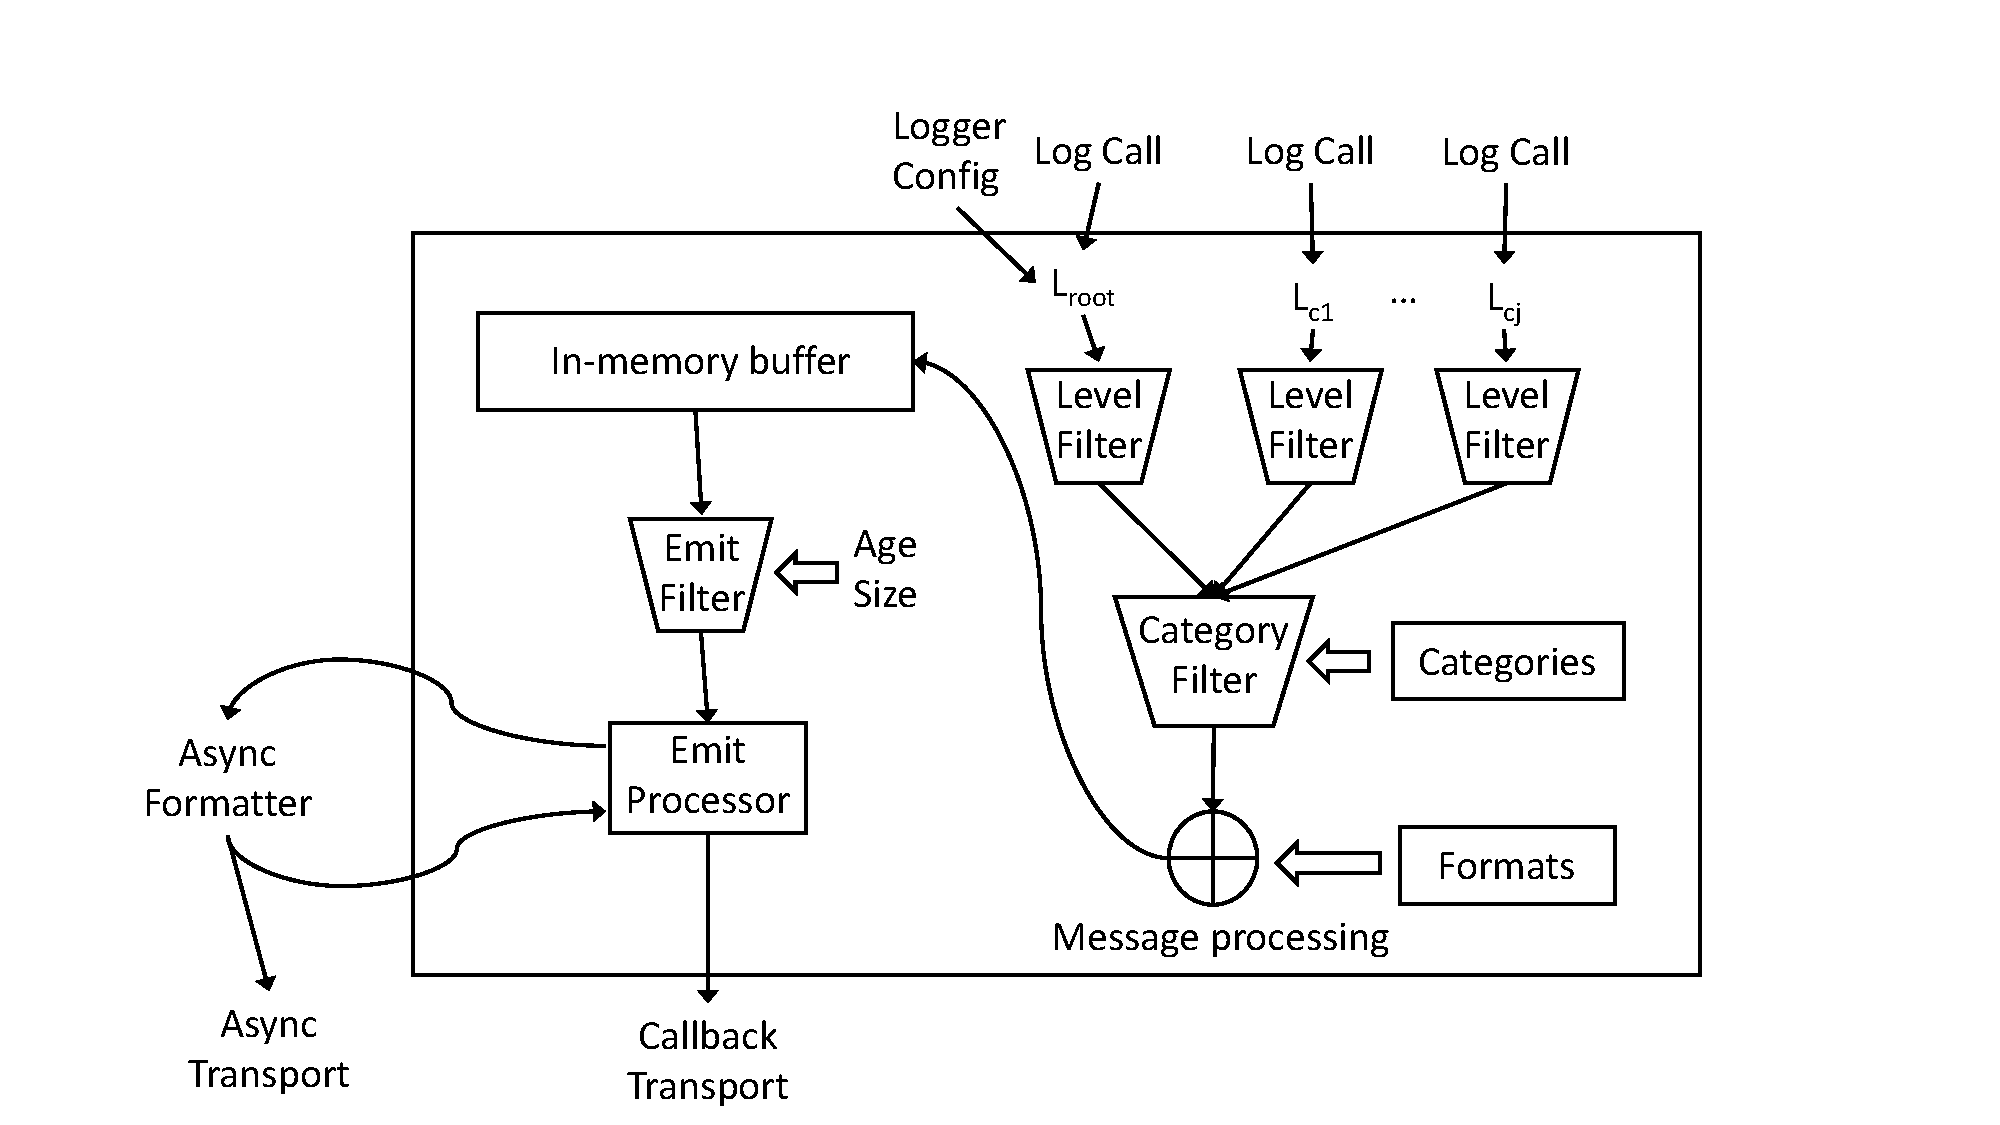
\includegraphics[width=0.5\textwidth,angle=-90]{Figures/ArchDiagram}
    \caption{Logger architecture}
    \label{fig:arch}
\end{figure}

\begin{figure*}[t]
\begin{minipage}[b]{0.47\textwidth}
    \lstinputlisting[language=JavaScript,basicstyle=\scriptsize]{Code/runningExample.js} 
    \caption{Main app code}
    \label{fig:appmain}
\end{minipage}
\begin{minipage}[b]{0.47\textwidth}
    \lstinputlisting[language=JavaScript,basicstyle=\scriptsize]{Code/runningExampleSub.js}
    \caption{Submodule code}
    \label{fig:appsub}
\end{minipage}
\caption{Running example}
\label{fig:runningExample}
\end{figure*}

\subsection{JavaScript Implementation}
\paragraph{Log State Manager}
\noindent
The first component we look at in the implementation is the global log state 
manager. This component is responsible for tracking all of the loggers that 
have been created, which is the root logger, the enabled logging levels + 
categories, and the message formats which have been defined. 

As seen in~\autoref{fig:arch} and the running example may be many loggers 
created in different parts of the application. One logger is created on line 
2 of the main application~\autoref{fig:appmain} while a second is created 
in the module \texttt{foo.js} in~\autoref{fig:appsub} which is included from 
the main \texttt{app.js} file. As stated in \emph{design principle 5} we 
do not want the included sub-module \texttt{foo.js} to be able to, unexpectedly, 
change the logging level for the main app (the call to \texttt{setOutputLevel} on 
line 9). We also want to allows the root logger to enable/disable log outputs 
from these subloggers.

To support these features the \projn logger keeps a list of all created loggers 
and a special \emph{root logger} which is the first logger created in the main 
module of the application. When updating logging levels or creating a new logger 
we check if action is comming from the root logger and, if not, either convert 
the call to a \texttt{nop} or look at the root logger configuration to see if 
we need to override any parameters.

In our running example the state manager will intercept the creation of the logger 
on line 2 in \texttt{foo.js}. Since the logger created here is not the root logger
the state manager will intercept this construction, set the in-memory log level to 
the overridden \texttt{WARN} level instead of the default value of \texttt{DETAIL}, 
prevent the modification of the \emph{emit-level} or the output sink, and will 
store the newly created logger in a list of sub-loggers. 

Tracking the list of all created sub-loggers also allows a developer to share a 
single logger between several files in the same module. The name parameter in the 
logger constructor is keyed with the logger and, if the same key is used in multiple 
places, the same logger object will be returned.

Finally, the state manager is responsible for maintaining information on the current 
\emph{emit level}, the enabled/disabled categories, and the sublogger override information. 
Each logger has an independent level at which it can write into the in-memory log but 
the state manager maintains a global set of enabled/disabled categories which each logger 
uses and a global logging level for eventual emit processing. Only the root logger is 
allowed to update the categories and emit levels. 

In our running example the main application has a log statement on lines $12$ and $14$ 
that are in the \texttt{Perf} category and will put a message with the current walltime 
in the log. As the first log statement happens before the \texttt{Perf} category has 
been enabled it will not be processed. However, after enabling the \texttt{Perf} category 
on line $13$ the log operation on line $14$ will be processed and result in a message 
being saved to the in-memory log.

\paragraph{Message Formats}
\noindent
To improve performance and enable the log output to be easily machine parsed we 
adopt a \emph{semantic logging} approach where the log call copies the format 
information and message arguments to a secondary location instead of formatting them 
immediately. Since the copy operation is very low cost this minimizes the 
performance impact on the main thread and allows the formatter to build up a 
parser for all the messages it emits which can be later used to parse the log. 
Modern software development also favors the use of consistent styles and data 
values in the log. Thus, \projn encourages developers to split the logging 
action into two components:
\begin{itemize}
\item Format definition using the \texttt{addFormat} method which takes a format 
string or JSON format object, processes it into an optimized representation, 
and then saves it for later use.
\item Format use in a log statment which takes a format identifier and a list of 
arguments, and then, processes them.
\end{itemize}

In addition to programtically processing single log formats, as shown on line 3 
in~\autoref{fig:appmain}, we also allow the programmer to load formats in bulk 
from a JSON formatted file. This allows a team to have a unified set of logging 
messages that can be loaded/processed quickly on startup and then used repeatedly 
throughout the applications execution. Once loaded all format objects are saved 
in the \emph{formats} component in~\autoref{fig:arch} where they can be loaded 
as needed for processing a log statement.

The format for a logger message is:
\begin{lstlisting}[language=JavaScript,basicstyle=\scriptsize]
{
  formatName: string, //name of the format
  formatString: string, //raw format string
  formatterEntries: {
    kind: number, //tag indicating the entry kind
    argPosition?: number, //position in argument list
    expandDepth?: number, //JSON expand depth
    expandLength?: number //JSON expand length
  }[]
}
\end{lstlisting}

This representation allows us to quickly scan an process the arguments as 
described in the \emph{Message In-Memory Processing} section. The kind 
information is used for both identifying what type of value is expected 
when formatting an argument, e.g. \texttt{number}, \texttt{string}, etc., 
but we also use it to support \emph{format macros}.

To support the easy/efficient logging on a number of common values that 
are not easily (or cheaply) computable we provide \emph{format macros}. 
Classic examples include adding the current walltime or the hostname as 
part of a log message. In JavaScript these require explicitly calling 
expensive compund API sequences \texttt{new Date().toISOString()} or 
\texttt{require('os').hostname()}. Instead we allow a developer to use 
special macros \texttt{\#walltime}, as seen on line 11 in~\autoref{fig:appmain}, 
or \texttt{\#host} in their format 
strings and then the logger has optimized internal paths to get the needed 
values. In these cases the \texttt{kind} field is set to the enumeration 
for the macro and the \texttt{argPosition} is undefined.

A common logging practice is to include raw objects, formatted as JSON, into the 
message. This is a convinient way to include rich data into a message but can 
lead to unexpectedly large logging loads when, what the developer expected to 
be a small object, turns out to be quite large. To prevent this we have a specialized 
JSON-style processor that will bound the depth/length of object expansion during 
formatting. The \texttt{expandDepth} and \texttt{expandLength} arguments provide 
control over this depth/length and can be adjusted in the format string when a 
developer want to capture more (or less) information than what is provided by the 
defaults.

\paragraph{Message In-Memory Processing}
\noindent
The in-memory buffer is implemented as a linked-list of block structures:
\begin{lstlisting}[language=JavaScript,basicstyle=\scriptsize]
{
  tags: Uint8Array,
  data: Float64Array,
  strings: string[],
  properties: map<number, string>
}
\end{lstlisting}

To allow efficient marshalling of the data from our JavaScript logger frontend 
to the C++ N-API code that handles the formatting we encode all values into 
$64$bit based representation (stored in the \texttt{data} property). We use a set 
of enumeration \texttt{tags} (stored in the \texttt{tags} property) to track 
what kind of value the corresponding $64$bit value represents. We have special 
handling for string and object properyt values, described below, that use the 
\texttt{strings} array and \texttt{properties} map to index and keep alive these values.

When implementing a sematic logging system the key invariant that needs to be 
preserved is that the values of each argument must not be changed between the 
time when the log call happens and when the argument is processed for 
formatting. Certain values including booleans, numbers, and strings, are 
immutable according to the language semantics so we can just copy the 
references directly into our in-memory array. However, in cases where the 
argument is a mutable object we must take explicit actions. A simple solution 
would be to JSON \texttt{stringify} the argument immedaitely, and while this 
prevents mutation and allows semantic formatting, it comprimises possible 
performance gains we are looking for. Instead we recursively flatten the object 
into the in-memory buffer with the code shown here:
\lstinputlisting[language=JavaScript,basicstyle=\scriptsize]{Code/flatten.js}

This code represents the transition from the \emph{formats} and \emph{arguments} 
inputs into the \emph{in-memory buffer} shown in~\autoref{fig:arch}. This code 
starts off by checking if we are either in a cycle or the depth bound has been 
reached. If either of these occour we put a special tag, \texttt{CycleTag} or 
\texttt{DepthBoundTag} respectively, into the tags array and return. If not we 
continue with the pre-order traveral of the object graph by updating the cycle 
info, adding the special \texttt{LParenTag} to the buffer, and enumerating the 
object properties. For each property we check if the length bound is met, adding 
the special \texttt{LengthBoundTag} and breaking if needed, if not we add the 
property and value information to the in-memory buffer. The property value \texttt{p} 
is a special string value which is very likely to be repeated so we use a map 
from properties to unique numeric identifiers to compress and convert them into 
a number which can be stored in the \texttt{data} component of the in-memory buffer 
via the \texttt{addPropertyEntry} function. The value associated is recursively 
processed via the \texttt{addGeneralEntry} call which switches on the type of the 
value, booleans and numbers are converted directly to \texttt{Float64} representations, 
strings are mapped by index in the \texttt{strings} array, and \texttt{Date} objects 
are converted to $64$bit timestamps using the \texttt{valueOf} method. Similar to 
standard JSON formatting other values are simplified but, instead of just dropping 
them, we use a special \texttt{OpaqueValueTag}. After all the properties have 
been processed we update the cycle tracking information and add a closing 
\texttt{RParenTag}.

\begin{figure}
    \centering
    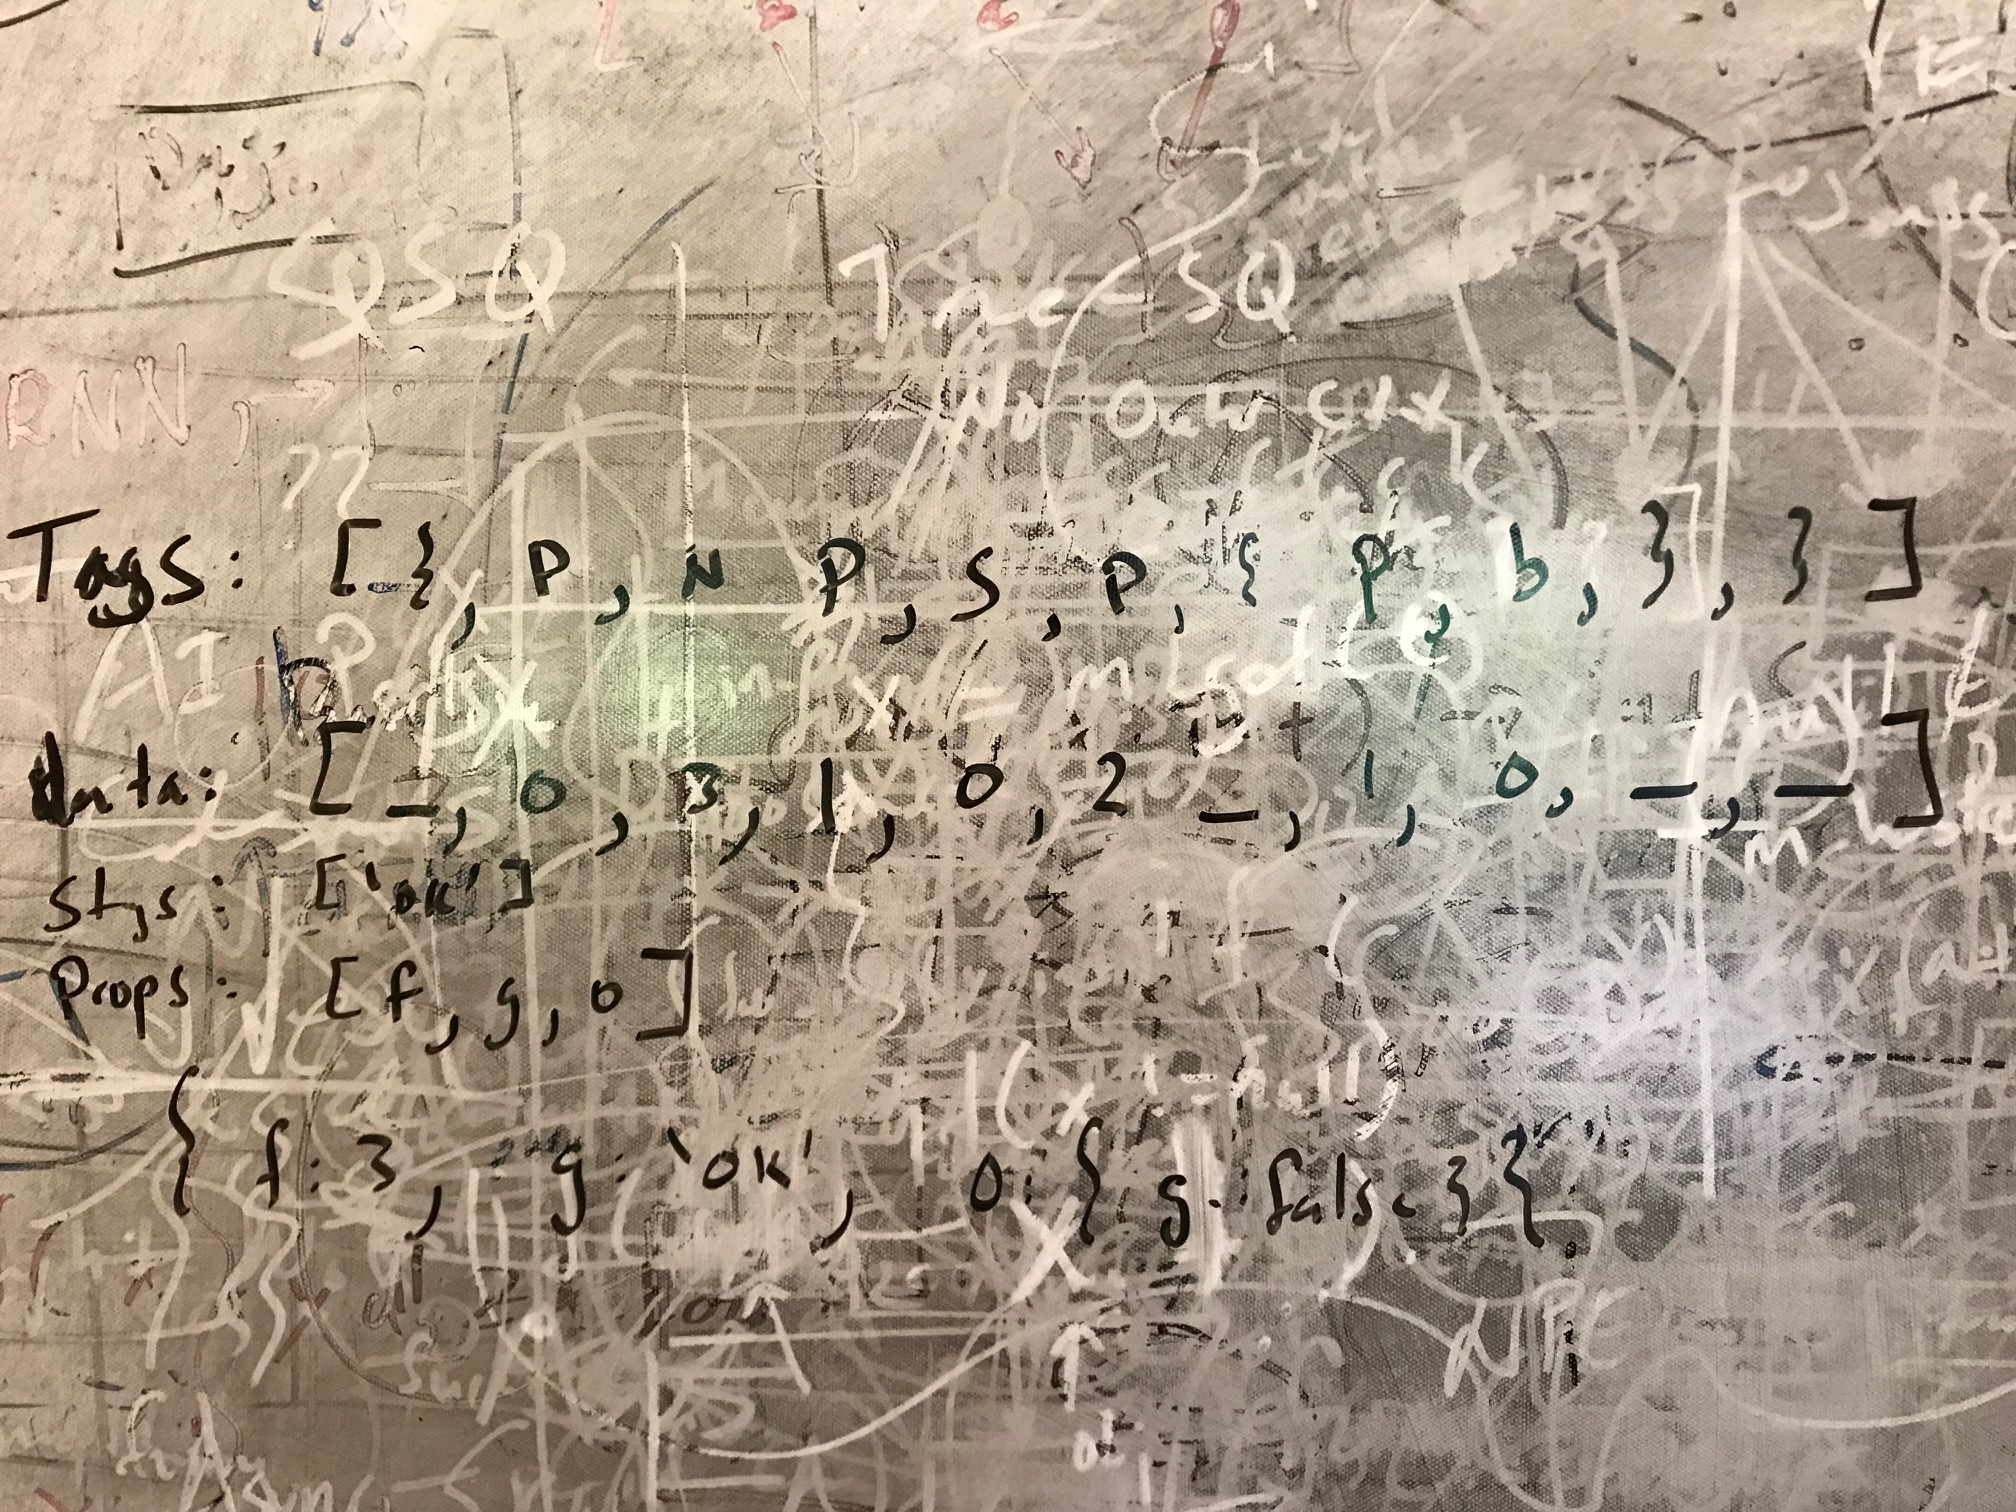
\includegraphics[width=0.5\textwidth]{Figures/InMemoryExample}
    \caption{In-Memory buffer processing example}
    \label{fig:inmemory}
\end{figure}

To illustrate how this code works in practice consider the case of processing the 
object argument:

\begin{lstlisting}[language=JavaScript,basicstyle=\scriptsize,numbers=none]
{
  f: 3,
  g: 'ok',
  o: { g: false, id: (x) => x }
}
\end{lstlisting}

The resulting state of the in-memory buffer is shown in~\autoref{fig:inmemory}. 
In this example we can see how the object structure has been flattened into 
the buffer with the \lstinline!'{'! and \lstinline!'}'! tags denoting the bounds 
of each object. Each of the properties has been registered in the map (with a fresh 
numeric identifier) and this is stored in the \texttt{data} array. For example the 
property \lstinline!g! is mapped to $1$ and in both occournces in the object 
structure the entry in the \texttt{tags} array is set to \lstinline!'p'! for 
property and the value in the \texttt{data} array is set to match the corresponding 
numeric identifier $1$. The numeric and boolean values are mapped in the obvious 
way, directly for the number and to $0$/$1$ for the boolean with the appropriate 
tag values set. Similar to the properties the string value \lstinline!'ok'! is 
mapped to an integer index, index $0$, in the \texttt{strings} array. Finally, 
since functions are not serializable, the value associated with the \lstinline!id! 
property is dropped and we simply store the \texttt{OpaqueValueTag} (\lstinline!'?'!) 
in the corresponding position of the \texttt{tags} array.

\paragraph{Message Staging and Emit}
\noindent

make sure to discuss callbacks + on demand synchrous emit

also detailed emit on "unusual" events

\paragraph{Logging APIs}
\noindent

\subsection{Native C++ Implementation}

Background N-API formatter

Background uploads

\subsection{Custom Runtime Implementation}

Format checking

Mutability checking

Code regen on level changes

Fast string + property handling



\section{Evaluation}
\label{sec:evaluation}
% !TeX root = Logpp.tex
Given the implementation of \projn from~\autoref{sec:implementation} we now shift 
to evaluating how well the resulting system meets the design goals outlined in~\autoref{sec:design}.\\

\noindent
For this evaluation we use four of microbenchmarks with $10$k iterations: 

\begin{lstlisting}[language=JavaScript,basicstyle=\scriptsize,numbers=none]
//Basic
log.info("hello world -- logger")
//String
log.info("hello %s", "world")
//Compound
log.info("hello %s %j %d", "world", { obj: true }, 4)
//Compute
log.info("hello at %j with %j %n -- %s", 
         new Date(), ["i", { f: i, g: "#" + i }], 
         i - 5, (i % 2 === 0 ? "ok" : "skip"))
\end{lstlisting}

\noindent
We also use a simple server based on the popular \emph{express}~\cite{} framework 
which provides a \emph{REST} API for querying data on the S\&P 500 companies.

All of the benchmarks are run on an Intel Xeon E5-1650 CPU with 6 cores at 3.50GHz, 32GB of RAM, and a SSD. 
The software stack is Windows 10 (17134) and Node v10.0.

\subsection{Microbenchmarks}
Our first evalaution is with current state of the art logging approaches in 
Node.js. These include the builtin \texttt{console} methods, the \texttt{debug}~\cite{debuglogger} 
module, the \texttt{bunyan}~\cite{bunyanlogger} logger, and the \texttt{pino}~\cite{pinologger} logger.

\begin{table}[t]  
    \centering
    \begin{tabular}{l | r r r r r | r }
    Program       & \bench{Basic}  & \bench{String}   & \bench{Compound}  & \bench{Compute} \\
    \hline
    Console       & $883$ms & $852$ms & $1064$ms & $986$ms \\
    Debug         & $202$ms & $200$ms & $282$ms  & $469$ms \\
    Bunyan        & $477$ms & $531$ms & $603$ms  & $920$ms \\
    Pino          & $188$ms & $190$ms & $296$ms  & $630$ms \\
    Log++         & $89$ms  & $93$ms  & $155$ms  & $304$ms \\
    \hline
    Speedup & $2.1$-$9.9\times$ & $2.0$-$9.2\times$ & $1.8$-$6.9\times$ & $2.1$-$3.2\times$ \\
    \end{tabular}
    \vspace{2mm}
    \caption{Timings for each logging framework on $10$k iterations with given format. 
    Speedup is the min-max speedup relative to the other logging frameworks.}
    \label{tab:microcompare}
\end{table}

The results in~\autoref{tab:microcompare} show the wide performance variation across logging 
frameworks (spanning nearly a factor of $10\times$). Accross all benchmarks \projn is consistently 
the fastest logger, by a factor of at least $1.8$-$2.1\times$, when compared to the best performing 
of the existing logging frameworks.

\subsection{Logging Optimization Impacts}
To understand how much each of our design choices and optimizations contributed to 
this performance we look at the performance impacts of specific features in \projn. 

\begin{table}[t]  
    \centering
    \begin{tabular}{l | r r r r r | r }
    Program       & \bench{Basic}  & \bench{String}   & \bench{Compound}  & \bench{Compute} \\
    \hline
    Enabled       & $883$ms & $852$ms & $1064$ms & $986$ms \\
    Disabled      & $883$ms & $852$ms & $1064$ms & $986$ms \\
    Sync-Lazy     & $202$ms & $200$ms & $282$ms  & $469$ms \\
    Sync-Strict   & $202$ms & $200$ms & $282$ms  & $469$ms \\
    Multi-Level   & $477$ms & $531$ms & $603$ms  & $920$ms \\
    \end{tabular}
    \vspace{2mm}
    \caption{ASDF}
    \label{tab:featureeval}
\end{table}

Lets do some microbencharks on logging and break down the impact of various 
implementation/design ideas...

enabled full

disabled

multi-level impact

expando impact

\begin{table}[t]  
    \centering
    \begin{tabular}{l | r r r r r | r }
    Program       & \bench{Host}  & \bench{App}   & \bench{Wallclock}  & \bench{Timestamp} \\
    \hline
    Explicit      & $883$ms & $852$ms & $1064$ms & $986$ms \\
    Expando       & $202$ms & $200$ms & $282$ms  & $469$ms \\
    \end{tabular}
    \vspace{2mm}
    \caption{ASDF}
    \label{tab:expando}
\end{table}

\subsection{Logging Performance}
Lets do some macro benchmarks on a couple of non-micro workloads to see the 
impact in practice...

No logging
----
Stat         Avg     Stdev   Max
Latency (ms) 0.14    0.55    38.43
Req/Sec      12011.1 2212.64 13170
Bytes/Sec    3.66 MB 678 kB  4.03 MB

132k requests in 11s, 40.4 MB read

console.log
----
Stat         Avg     Stdev   Max
Latency (ms) 1.18    0.83    48.53
Req/Sec      6038.3  1082.77 6668
Bytes/Sec    1.84 MB 328 kB  2.04 MB

60k requests in 10s, 18.5 MB read

pino         
----
Stat         Avg     Stdev  Max
Latency (ms) 0.89    0.7    39.69
Req/Sec      8133.3  1457.5 8861
Bytes/Sec    2.49 MB 441 kB 2.71 MB

81k requests in 10s, 24.9 MB read

Logpp detail 
----
Stat         Avg     Stdev   Max
Latency (ms) 0.67    0.8     42.78
Req/Sec      8645.1  1656.58 9784
Bytes/Sec    2.64 MB 503 kB  2.99 MB

86k requests in 10s, 26.4 MB read

logpp info   
----
Stat         Avg     Stdev   Max
Latency (ms) 0.58    0.77    43.77
Req/Sec      8958.55 1654.89 10075
Bytes/Sec    2.75 MB 508 kB  3.08 MB

99k requests in 11s, 30.1 MB read

\subsection{Logging Data Size}

study of simplified output log and reduction in storage/transport sizes -- 
e.g., save XXMB of traffic/storage per day kind of thing.

compression impact


\section{Conclusion}

\section{Notes} log output scheduling -- critical for devops/cloud integration
-- should be background task


\balance

{
\raggedright 

\bibliographystyle{abbrv}
\bibliography{bibfile} 
}


\end{document}
